% Source of the figures of knot-theory.tex.
% Each tikzpicture is one page. Build (out of
% this folder, into some build directory B):
%   pdflatex -output-directory=B figures.tex
%   gs -q -dNOPAUSE -dBATCH -sDEVICE=png16m \
%     -r220 -dTextAlphaBits=4 \
%     -dGraphicsAlphaBits=4 \
%     -sOutputFile=B/fig-%d.png B/figures.pdf
% then copy fig-1..5 here as crossing-signs,
% smoothings, reidemeister, trefoil-braid,
% torus-square.
\documentclass[tikz,border=4pt]{standalone}
\usetikzlibrary{arrows.meta}
\tikzset{
  strand/.style={line width=1.1pt},
  over/.style={line width=1.1pt,
    preaction={draw,white,line width=6pt}},
  arr/.style={-{Stealth[length=6pt]}},
}
\begin{document}

% page 1: crossing signs
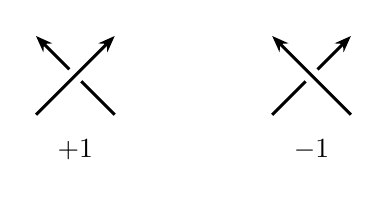
\begin{tikzpicture}
\draw[strand,arr] (1,0) -- (0,1);
\draw[over,arr] (0,0) -- (1,1);
\node at (0.5,-0.45) {$+1$};
\begin{scope}[xshift=3cm]
\draw[strand,arr] (0,0) -- (1,1);
\draw[over,arr] (1,0) -- (0,1);
\node at (0.5,-0.45) {$-1$};
\end{scope}
\end{tikzpicture}

% page 2: the two smoothings
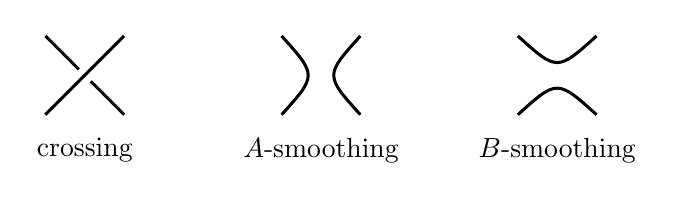
\begin{tikzpicture}
\draw[strand] (1,0) -- (0,1);
\draw[over] (0,0) -- (1,1);
\node at (0.5,-0.45) {crossing};
\begin{scope}[xshift=3cm]
\draw[strand] (0,0) .. controls (0.45,0.5)
  .. (0,1);
\draw[strand] (1,0) .. controls (0.55,0.5)
  .. (1,1);
\node at (0.5,-0.45) {$A$-smoothing};
\end{scope}
\begin{scope}[xshift=6cm]
\draw[strand] (0,0) .. controls (0.5,0.45)
  .. (1,0);
\draw[strand] (0,1) .. controls (0.5,0.55)
  .. (1,1);
\node at (0.5,-0.45) {$B$-smoothing};
\end{scope}
\end{tikzpicture}

% page 3: Reidemeister moves
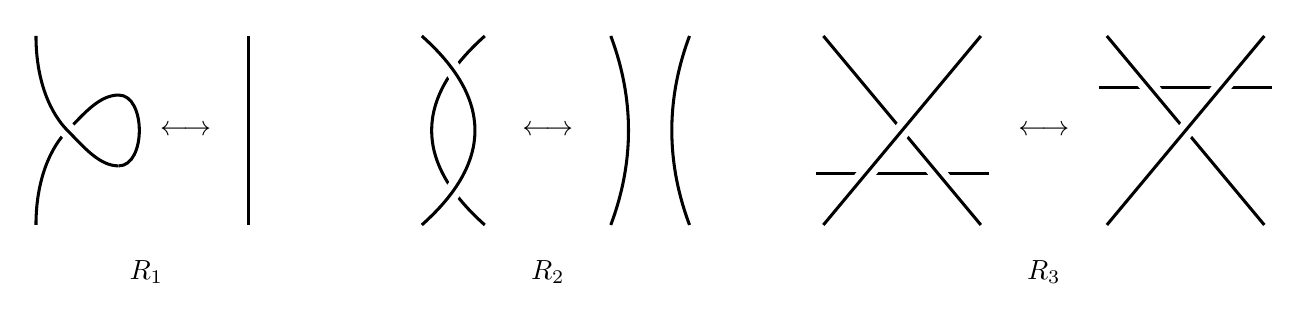
\begin{tikzpicture}
% R1: a kink
\draw[strand] (0.2,-0.2)
  .. controls (0.2,0.4) and (0.4,0.8)
  .. (0.6,1.0)
  .. controls (0.8,1.2) and (1.0,1.45)
  .. (1.25,1.45)
  .. controls (1.6,1.45) and (1.6,0.55)
  .. (1.25,0.55);
\draw[over] (1.25,0.55)
  .. controls (1.0,0.55) and (0.8,0.8)
  .. (0.6,1.0)
  .. controls (0.4,1.2) and (0.2,1.6)
  .. (0.2,2.2);
\node at (2.1,1) {$\longleftrightarrow$};
\draw[strand] (2.9,-0.2) -- (2.9,2.2);
\node at (1.6,-0.8) {$R_1$};
% R2
\begin{scope}[xshift=5cm]
\draw[strand] (0.9,-0.2) .. controls (0,0.6)
  and (0,1.4) .. (0.9,2.2);
\draw[over] (0.1,-0.2) .. controls (1,0.6)
  and (1,1.4) .. (0.1,2.2);
\node at (1.7,1) {$\longleftrightarrow$};
\draw[strand] (2.5,-0.2) .. controls
  (2.8,0.6) and (2.8,1.4) .. (2.5,2.2);
\draw[strand] (3.5,-0.2) .. controls
  (3.2,0.6) and (3.2,1.4) .. (3.5,2.2);
\node at (1.7,-0.8) {$R_2$};
\end{scope}
% R3: the horizontal strand lies below the
% other two and slides across their crossing
\begin{scope}[xshift=10.2cm]
\draw[strand] (-0.1,0.45) -- (2.1,0.45);
\draw[over] (2,-0.2) -- (0,2.2);
\draw[over] (0,-0.2) -- (2,2.2);
\node at (2.8,1) {$\longleftrightarrow$};
\begin{scope}[xshift=3.6cm]
\draw[strand] (-0.1,1.55) -- (2.1,1.55);
\draw[over] (2,-0.2) -- (0,2.2);
\draw[over] (0,-0.2) -- (2,2.2);
\end{scope}
\node at (2.8,-0.8) {$R_3$};
\end{scope}
\end{tikzpicture}

% page 4: closure of three positive crossings
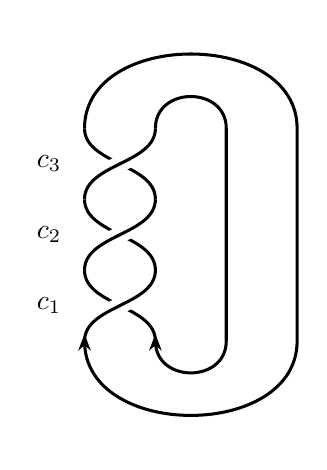
\begin{tikzpicture}[scale=0.9]
\foreach \k in {0,1,2} {
  \draw[strand] (1,\k) .. controls (1,\k+0.5)
    and (0,\k+0.5) .. (0,\k+1);
  \draw[over] (0,\k) .. controls (0,\k+0.5)
    and (1,\k+0.5) .. (1,\k+1);
}
\draw[strand] (1,3) .. controls (1,3.6)
  and (2,3.6) .. (2,3) -- (2,0)
  .. controls (2,-0.6) and (1,-0.6) .. (1,0);
\draw[strand] (0,3) .. controls (0,4.4)
  and (3,4.4) .. (3,3) -- (3,0)
  .. controls (3,-1.4) and (0,-1.4) .. (0,0);
\draw[strand,arr] (0,-0.03) -- (0,0.1);
\draw[strand,arr] (1,-0.03) -- (1,0.1);
\node at (-0.5,0.5) {$c_1$};
\node at (-0.5,1.5) {$c_2$};
\node at (-0.5,2.5) {$c_3$};
\end{tikzpicture}

% page 5: the curve (2,3) on the square
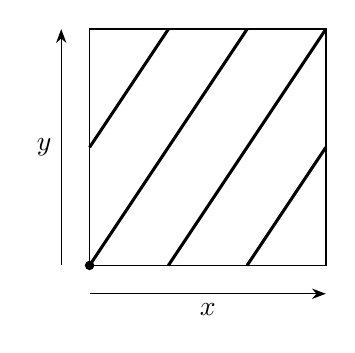
\begin{tikzpicture}[scale=3]
\draw[line width=0.6pt] (0,0) rectangle (1,1);
\draw[strand] (0,0) -- (0.6667,1);
\draw[strand] (0.6667,0) -- (1,0.5);
\draw[strand] (0,0.5) -- (0.3333,1);
\draw[strand] (0.3333,0) -- (1,1);
\draw[-{Stealth[length=5pt]}] (0,-0.12)
  -- (1,-0.12) node[midway,below] {$x$};
\draw[-{Stealth[length=5pt]}] (-0.12,0)
  -- (-0.12,1) node[midway,left] {$y$};
\fill (0,0) circle (0.02);
\end{tikzpicture}

\end{document}
